%!TeX TXS-program:bibliography = txs:///biber
\documentclass{article}
\usepackage[utf8]{inputenc}
\usepackage{booktabs, float, color, colortbl, graphicx, ragged2e, setspace, threeparttablex, threeparttable, longtable, placeins, booktabs, float, tabularx}
\usepackage[english]{babel}
\usepackage{adjustbox}
\usepackage{acronym}
\usepackage{csquotes}
\usepackage[plainpages=false]{hyperref}
\usepackage{todonotes}

\hypersetup{%
	%backref=true,%
    plainpages=false,%
	naturalnames=true,%
	bookmarksnumbered=true,%
	bookmarksopen=false,%
	plainpages=true,%
	colorlinks=true,%
	urlcolor=black,
	linkcolor=black,%
	filecolor=black,%
	citecolor=black,%
	%pagecolor=myblue,%
	%pdftitle={\mytitle},%
	pdfpagemode=UseOutlines%
	%pdfauthor={\myauthors},%
	%pdfsubject={\myshorttitle}
}
\usepackage[natbib]{biblatex}

% bibliography
\addbibresource{paper.bib}

\acrodef{CDER}{Canadian Center for Data Development and Economic Research}
\acrodef{PEI}{Prince Edward Island}
\acrodef{LEAP}{Longitudinal Employment Analysis Program}

\newcommand{\sym}[1]{\rlap{#1}}
\title{Synthetic Data for Canadian Longitudinal Business Data }
\author{M. Jahangir Alam, Benoit Dostie, Lars Vilhuber}
\begin{document}
\maketitle
\setstretch{1.5}
\begin{abstract}
\noindent
=======
Data on businesses collected by statistical agencies are challenging to protect. Many businesses have unique characteristics, distributions of employment, sales, and profits are highly skewed, and  most disclosure avoidance mechanisms  fail to strike an acceptable balance between usefulness and confidentiality protection. Often, only very few aggregate statistics are released, and access to confidential microdata can be burdensome.

%Statistics Canada collects data and creates databases based on administrative records on business establishments and enterprises, however, they only disseminate those business databases in highly aggregated forms. Since it is costly and inconvenient for researchers to get access to Canadian micro business databases, 
This paper documents the creation of a synthetic data version of Statistics Canada's Longitudinal Employment Analysis Program (LEAP). Since the LEAP has a structure similar to the U.S. Longitudinal Business Database (LBD), this allows us to adapt the procedures that were used by {add citation} to create the synthetic LBD in a Canadian context. We show the synthetic LEAP is analytically valid for a wide range of commonly used statistical analyses, while maintaining respondents' confidentiality.
% by Lars: We document an experiment to create an analytically valid synthetic version of the Longitudinal Employment Analysis Program (LEAP). We implement the algorithm used by \cite{RePEc:bla:istatr:v:79:y:2011:i:3:p:362-384}, with minor adjustments. We document the analytical validity for various typical uses, as well as provide evidence of the  confidentiality of the database.


\end{abstract}
\newpage
\tableofcontents
\newpage
\section{Introduction}
%Statistics Canada collects data and creates databases based on administrative records (like T4 slip that is the annual statements of remuneration paid) on business establishments and enterprises, however, they only disseminate those business databases in highly aggregated forms into two-digit industry categories. The \acf{CDER} in Statistics Canada is responsible to protect the confidentiality of business data. \ac{CDER} does not disseminate those business databases for two reasons. First, a confidentiality breach related to the business database is potentially more damaging to the statistical system because of the importance of key respondents that are more likely to be identifiable, e.g. Bombardier inc., a company mainly specializing in air and railway technology or Cavendish farm in \ac{PEI}. Second, the financial gains related to identifying a respondent are potentially greater, for example, people could make a profit by in investing stock markets through identifying Bombardier Inc. 
While Canada maintains a network of research data centers similar to the one in the U.S., there is virtually no firm-level data sets amongst the data holdings of the Canadian Research Data Center Networks (CRDCN). Researchers who need access to confidential micro-level business data have to go to the Canadian Center for Data Development and Economic Research (CDER) located in the headquarters of Statistics Canada. One reason commonly heard for this limited access has to do with the fact that Canada is a small country with a highly skewed distribution of firms, thus compounding problems linked to confidentiality protection. 

%To give access to business databases, CDER currently uses three measures in place to mitigate the higher risk to the statistical system when business microdata are accessed. First, a batch-submit system is used when accessing the actual data. Second, actual individual observations cannot be accessed without it being recorded. Third, ``CDER version of synthetic data'' is also provided to aid with programming.
Confidentiality protection with CDER is done through a variety of means, including remote execution and research monitoring. But more importantly, researchers accessing CDER data holdings must become \textit{deemed employees} of Statistics Canada and sign an asset-freeze agreement to ensure they do not profit financially from their research.

%Since it is costly and inconvenient for both researchers and Statistics Canada to get access to business databases, in this project, we create synthetic data\footnote{Synthetic data are created by replacing sensitive values with repeated draws from a model fit to the original data (Little, 1993; Rubin, 1993). This approach is closely related to multiple imputations.} for Canadian LEAP database during the period of 1991 to 2014 using 2015 LEAP vintage. In this project, we have three objectives: i) evaluate to what extent synthetic code developed for the U.S. Longitudinal Business Database (LBD) can easily transferable to LEAP database with comparable structure; ii) examine whether the automated synthesis will generate useful datasets that offer analytical validity for a wide range of statistical analyses; iii) provide evidence on confidentiality properties. 
Since 2018, Statistics Canada has undertaken a so-called Modernization initiative. One of the objective of that Initiative is to improve access to researchers to confidential firm-level micro data. As part of this initiative, we have been asked by CDER to explore how the creation of synthetic data could help achieve part of that objective. Synthetic data are created by replacing sensitive value from the original data with repeated draws from a model fit to the original data (Little, 1993; Rubin, 1993). This approach is closely related to multiple imputations. 

% by Lars: The situation described above for access to Canadian business microdata is not unique. Drechsler (CITE) and \cite{RePEc:bla:istatr:v:79:y:2011:i:3:p:362-384} have proposed solutions based on the creation of synthetic business microdata.\footnote{Synthetic data are created by replacing sensitive values with repeated draws from a model fit to the original data (Little, 1993; Rubin, 1993). The approach is closely related to multiple imputations.} In the latter case, access to the synthetic data is combined with a validation server (CITES). 

% by Lars: To reduce the cost of granting and obtaining access to the Canadian business microdata, we created  synthetic data for the  \ac{LEAP} database. In this project, we have three objectives: i) evaluate to what extent synthetic code developed for the U.S. Longitudinal Business Database (LBD) can easily transferable to LEAP database with comparable structure; ii) examine whether the automated synthesis will generate useful datasets that offer analytical validity for a wide range of statistical analyses; iii) provide evidence on confidentiality properties. 

%Synthetic code developed for the U.S. LBD can easily transferable to Canadian LEAP database with comparable structure, however, there are some issues raised to implement that the U.S. synthetic code in Canadian LEAP database. First, the U.S. synthetic LBD code does not converse for a group of industries for each time of implementation. Second, the U.S. synthetic LBD code does not properly approximate the last year information of firms. Third, the U.S. synthetic LBD code generates, in some cases, zero employment or payroll during the life cycles of firms.   
We use this approach on the Canadian Longitudinal Employment Analysis Program (LEAP) 2015 that contains retrospective data on firms from 1991 to 2014. Our implementation adapts the approach used to create synthetic data version of the Longitudinal Business Database (LBD) from the United States since both data sets have a similar structure and are used for similar research questions. We assess the performance of the newly created synthetic along two dimensions: analytical validity and confidentiality protection.

%Canadian synthetic database generates analytical validity for a wide range of statistical analysis which commonly uses in the literature. For example, we find that firm characteristics (gross employment, total payroll, the share of firms, the share of employment, the share of payroll) in the Canada synthetic data are very close to those in the LEAP, however, the manufacturing sector shows more close pattern than the private sector.  In addition, we compare firm dynamics (entry and exit rates) and dynamics of job flows (job creation rate, and net job creation rate) between Canadian synthetic and LEAP database and find that those firm dynamics are similar. Furthermore, we assess how well Canadian database captures variability in economic growth due to industry and firm age using several dynamic panel data models and find that Canadian synthetic database provides similar predictions to LEAP database. 
We verify the analytical validity of synthetic data set so created along a variety of measures. First, we show that more average firm characteristics (gross employment, total payroll) in the synthetic data closely match those from the original data. Second, we also find the synthetic data close replicates various measures of firm dynamics (entry and exit rates) and job flows (gross and net job creation rate) from the original data. Finally, we assess whether measures of economic growth vary between both data sets using a dynamic panel data models and find that both data sets yield similar predictions.

%To provide evidence on confidentiality properties of Canadian synthetic database, we estimate the probability that the synthetic first year equals the true first year given the synthetic fist year and find that those probabilities are quite low except for the first year of LEAP database. This is because of censoring and lack of previous information. 
To provide evidence on the confidentiality properties this newly created  synthetic database, we estimate the probability that the synthetic first year equals the true first year given the synthetic fist year and find that those probabilities are quite low except for the first year of LEAP database. This is because of censoring and lack of previous information.\todo{BD: I have no idea what this means, please explain better.}

%This paper is organized as follows. Section 2 includes a detailed description of the LEAP database and usages of LEAP database. Section 3 provides a brief overview of the evolution of synthetic data and implementation in the Canadian context. In section 4, the analytical validity of synthetic database is discussed. Finally, this paper concludes in Section 5. In addition, it includes a description to include other variables in Canadian synthetic database as an extension.
The rest of the paper is organized as follows. Section 2 provides a detailed description of the LEAP database and its uses. Section 3 defines what we mean by synthetic data and describe how we created the synthetic LEAP. In section 4, the analytical validity of synthetic database is assessed. Section 5 concludes.

\section{Data Description}

\subsection{LEAP database}

The LEAP contains information on annual employment for each employer in Canada. It covers incorporated and unincorporated businesses that issue at least one annual statements of remuneration paid (T4) in any given calendar year, but excludes self-employed individuals or partnerships with non-salaried participants. One advantage of the LEAP is that it covers all sectors of the economy.% - though some of the information is more meaningful for the business sector than the public sector.

To construct the LEAP Statistics Canada draws from three distinct sources: (1) T4 statements from Canada Revenue Agency, (2) Statistics Canada's Business Register, and (3) Statistics Canada's Survey of Employment, Payrolls and Hours (SEPH). In Canada, employing businesses are required to register with Canada Revenue Agency using their Business Number, and issue to each of their employees a T4 statement summarizing earnings received in the current year. This process creates a link between the employee and the business through the Business Number that is the backbone of LEAP. Reported payrolls from SEPH allows estimates of annual employment to be added to the data set. The payroll is converted to employment (called ALUs or Average Labour Units, defined later) using conversion factors derived from the SEPH. 

The LEAP essentially contains four variables (1) A Longitudinal Business Register Identifier (LBRID), (2) Industry, (3) Employment and (4) Payroll. This still allows research on multiple themes, like employment growth, industry turnover, firm survival, job creation and job destruction, etc. We discuss each of those variables in turns. 

\textbf{LBRID:} This is the unique identifier assigned to each enterprise.  The LBRID tracks the enterprise across all years in which it has employees, for the period covered by the LEAP vintage. It is derived from the Business Register enterprise identifier (BRID). 

For various administrative reasons, an enterprise's identifier in the Business Register may sometimes change from year to year.  This would lead to the appearance of false deaths and births in the LEAP file.  To avoid this, a system of Labour Tracking is used to track the movements of workers between firms.  This is used to detect false births and deaths and link firms by a common LBRID. Labour tracking can lead to many different types of linkages between firms. 

The simplest would be a one-to-one linkage between a death and a birth record. For example, if a business changes from incorporated to limited business, the Business Register may remove the original business from the register and create a new one. In this case, the only action necessary is to assign a common LBRID to the two businesses over time. 

A more complex case would be a merger between two firms, where most employees from the previous two firms are at a new firm. Here, all three entities are given the same LBRID, and the past records of the two merged firms would be combined into a single record. The employment of the two firms is added together, and the current NAICS code for the new firm is assigned to the combined, synthetic past record. In other words, it would be as if the newly merged firm already existed in the past. Similarly, acquisitions and spin offs lead to the combination of firms and the creation of synthetic records. 

\textbf{Industry:} The 4-digit North American Industrial Classification System (NAICS) code that is assigned to a firm nationally. This is the dominant NAICS code for firms that have activity in multiple industries. One of the characteristics of the LEAP is that the industry code for the most recent year that the firm is in operation is pushed back in time, so that an enterprise has the same industry code each year within the same vintage.  

\textbf{Employment:} Employment of each firm is measured by its average labour units (ALUs). ALUs are the average employment an enterprise would have if it paid its workers the average annual earnings (AAE) of a typical worker in the enterprise's particular industry, province and enterprise size class. AAE are derived using information from the SEPH.

\textbf{Payroll:} Sum of payroll from all T4 slips issued by the enterprise.
We next turn to the methods we used to create a synthetic version of the LEAP.

\section{Methodology}

\subsection{Overview}

There is growing demand for firm-level data allowing detailed studies of firm dynamics. Recent examples include \textcite{NBERc0480} who use cross-country firm-level data to study average post-entry behavior of young firms. \textcite{10.1257/aer.20141280} use the BDS \todo{BD: define BDS} to show the role of firm size in firm dynamics. % but also had access to the Synthetic LBD. 

However, such studies are made difficult due to the limited or restricted access to firm-level data.% across countries and also within-country, it is difficult to identify the sources of the variation in firm dynamics across countries. 
To provide better access to establishment data in the United States, \textcite{RePEc:bla:istatr:v:79:y:2011:i:3:p:362-384} describe an approach to create and release synthetic data for Longitudinal Business Database (LBD), which was created in the early 2000s (see \textcite{RePEc:cen:wpaper:02-17} for details). The variables currently available in the LBD are industry, annual payroll, employment, geography, birth year, death year, and firm structure\todo{BD: can we be more precise than geography and firm structure?}.    

We can currently distinguish between two methods to create synthetic data. The general approach to data synthesis is to generate a joint posterior predictive distribution of $Y|X$ where $Y$ are variables to be synthesized and $X$ are unsynthesized variables. In the Phase 1 version of the method, variables are synthesized in a sequential fashion, with categorical variables being generally processed first using a variant of Dirichlet-Multinomial. Continuous variables are then synthesized using a normal linear regression model with kennel density-based transformation (\textcite{WOODCOCK20094228}). 

The Phase 2 version of the method has shifted to a Classification and Regression Trees (CART) model with Bayesian bootstrap. For the United States, the phase 2 version  is currently in its final stages of implementation (\textcite{RePEc:cen:wpaper:14-12}). 

To evaluate whether synthetic data algorithms developed in the U.S. can be adapted to generate similar synthetic data for other countries, \textcite{RePEc:cen:wpaper:14-13} implement the Phase 1 version of the method to the German Longitudinal Business Database (GLBD). 

\subsection{Implementation in the Canadian context}

To create a Canadian synthetic database, we use the 2015 LEAP vintage. As for the U.S. synthetic database for LBD,\todo{BD: Is the name SynLBD official, and should we use it?} we synthesize categorical variables first, followed by continuous variables, controlling for the firm ID and industry classification at 4-digit NAICS (see Table~\ref{tab:LEAP_Variable}.)

% Table tab:LEAP_Variable
\begin{table}[H]
  \centering\footnotesize
  \caption{CanSynLEAP variable descriptions}  \label{tab:LEAP_Variable} \medskip
  \renewcommand{\arraystretch}{1}
  \begin{tabular}{l  c c c c c}
    \toprule
    \textbf{Name}&\textbf{Type}&\textbf{Description}&\textbf{Notation}&\textbf{Action}\\
    \midrule
synid&Identifier&Unique random number for enterprise&&Created\\
NAICS&Categorical&4 digit industry code&$x_{1}$&Unmodified\\
Firstyear&Categorical&First year enterprise is observed &$y_{1}$&Synthesized\\
Lastyear&Categorical&Last year enterprise is observed &$y_{2}$&Synthesized\\
Year&Categorical&Year dating of annual variables&&Created\\
ALU&Continuous&(annual)&$y_{3}$&Synthesized\\
Payroll&Continuous&Payroll (annual)&$x_{4}$&Synthesized\\
   \bottomrule
  \end{tabular} 
\\
Note: Variables denoted with $y_{i}$ are synthesized and variables denoted with $x_{i}$ are not synthesized. 
\end{table}

After implementing the U.S. synthetic LBD code, we follow four steps to create a Canadian synthetic database. \begin{enumerate}
    \item We exclude the public sector (NAICS 61, 62, and 91) because Statistics Canada does not produce any statistics for those sectors.
    \item We exclude industries for which the algorithm is not converging.% for each time of implementation of the U.S. synthetic code for LBD. 
    These industries are NAICS 4481,    4482,     4483,     4511,     4513,     4841,     4842,     5241, and 5242. These industries represent approximately 7 percent of the total number of observations and are labeled as ``not synthesized'' in Table \ref{Synthesized_observations}.
    \item We drop some industries, from the synthesized industries, which have sensitive information.\todo{Which one? What is meant by sensitive?}
    \item We drop observation for the last year each firm was observed since the SynLBD code does not properly approximate the last year of the data.
\end{enumerate}. 
After the implementation of these steps, we have around 22 million observations in the CanSynLBD database during the period of 1991 - 2014.\todo{Need to mention suppressed industries. Note presence of 0000 industries. Discuss.}

\begin{table}[H]
  \centering
\begin{threeparttable}
  \caption{Synthesized observations}  \label{Synthesized_observations} \medskip
  \renewcommand{\arraystretch}{1}
  \begin{tabular}{l  c c }
    \toprule
    \textbf{Category}&\textbf{\# of Observations (millions)}&\textbf{Percentage}\\
    \midrule
Synthesized&22.01&93.35\\
Not synthesized&1.57&6.65\\
Total&23.58&100.00\\

   \bottomrule
  \end{tabular} 
\begin{tablenotes}
\small
\item Note: Not synthesized industries are NAICS 4481,    4482,     4483,     4511,     4513,     4841,     4842,     5241, and 5242. These industries are not converging for each time of implementation We drop industries, from the synthesized industries, which have sensitiveness information.\todo{BD: adjust footnote using previous answers to questions.} We do not synthesize the public sector (NAICS 61, 62, and 91).
 \end{tablenotes}
 \end{threeparttable}
\end{table}

%\newpage

\section{Analytical validity}

\subsection{Firm Characteristics}

The CanSynLBD and LEAP generally provide comparable inferences on aggregate means and correlations. For example, Figures \ref{GrossEmploymentPrivate} and \ref{GrossEmploymentManufacturing} show that gross employment levels for each year in the CanSynLBD are very close to those in the LEAP. However, the manufacturing sector shows closer patterns than private sector.\todo{BD: Is what is included in the Private sector defined somewhere? Is the Manufacturing sector included in the Private sector? Please provide details} We find similar results for total payroll (Figures \ref{TotalPayrollPrivate} and  \ref{TotalPayrollManufacturing}) .\todo{Redo Graph \ref{GrossEmploymentPrivate} omitting the last year}

\todo{Why is manufacturing always below, but overall employment crosses? Which industries are driving that?}
\begin{figure} [H]
\centering
\caption{Gross employment level by year (private)} \label{GrossEmploymentPrivate}
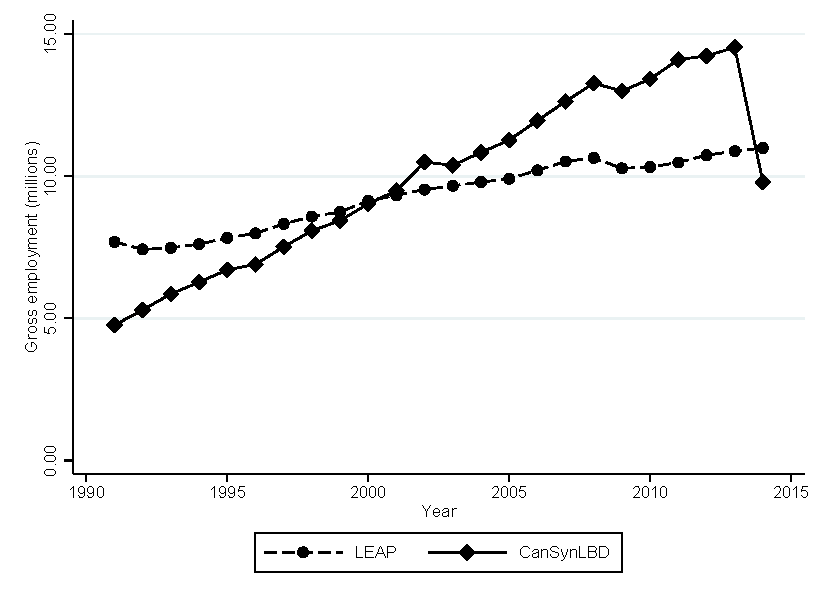
\includegraphics[height=2.8in, width=.7\linewidth]{graphs/Gross_employment_level_by_year_private_bw.pdf} 
\begin{minipage}{0.85\textwidth}
{\footnotesize Note: $LEAP$ is the Longitudinal Employment Analysis Program and $CanSynLBD$ is the Canadian synthetic database based on LEAP. In this graph, we use the 2015 vintage of LEAP for private sector and drop the last year of observation for each firm. \par}
\end{minipage}
\end{figure}


\begin{figure} [H]
\centering
\caption{Gross employment level by year (manufacturing)} \label{GrossEmploymentManufacturing}
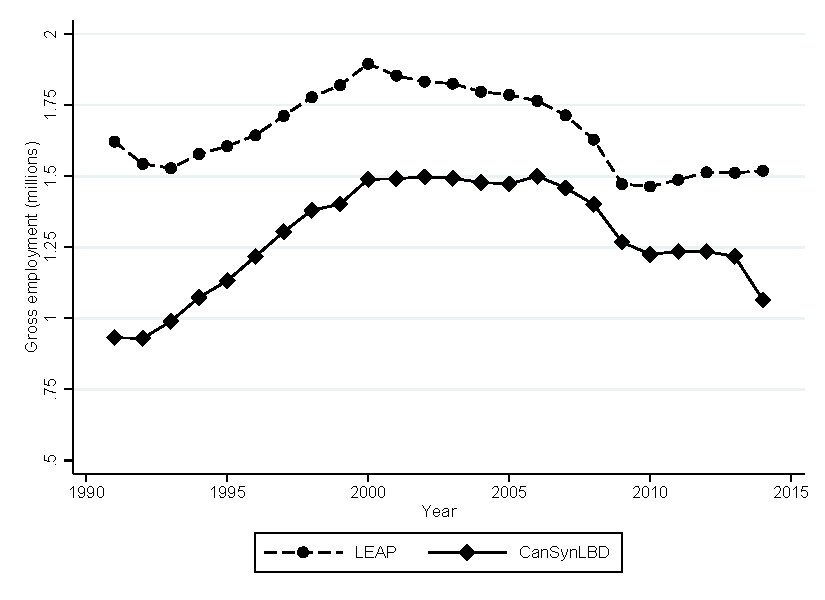
\includegraphics[height=2.8in, width=.7\linewidth]{graphs/Gross_employment_level_by_year_manufacturing_bw.pdf} 
\begin{minipage}{0.85\textwidth}
{\footnotesize Note: $LEAP$ is the Longitudinal Employment Analysis Program and $CanSynLBD$ is the Canadian synthetic database based on LEAP. In this graph, we use the 2015 vintage of LEAP for the private sector and drop the last year of observation for each firm. \par}
\end{minipage}
\end{figure}


\begin{figure} [H]
\centering
\caption{Total payroll by year (private)} \label{TotalPayrollPrivate}
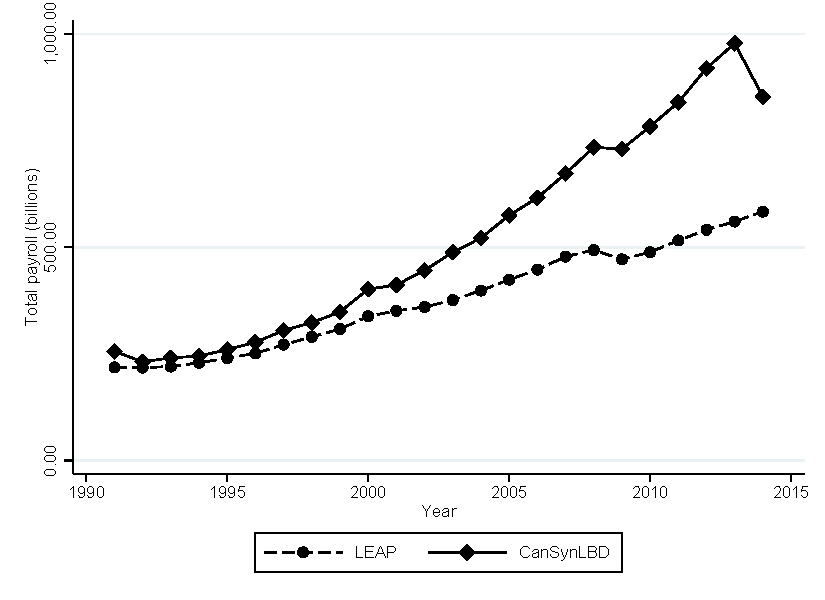
\includegraphics[height=2.8in, width=.7\linewidth]{graphs/Total_payroll_by_year_private_bw.pdf} 
\begin{minipage}{0.85\textwidth}
{\footnotesize Note: $LEAP$ is the Longitudinal Employment Analysis Program and $CanSynLBD$ is the Canadian synthetic database based on LEAP. In this graph, we use the 2015 vintage of LEAP for the private sector and drop the last year of observation for each firm. \par}
\end{minipage}
\end{figure}
\begin{figure} [H]
\centering
\caption{Total payroll by year (manufacturing)} \label{TotalPayrollManufacturing}
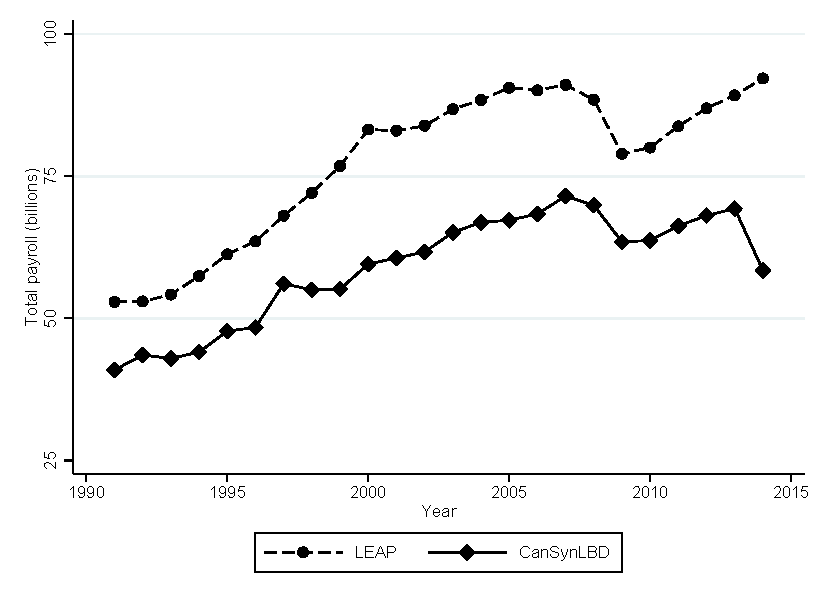
\includegraphics[height=2.8in, width=.7\linewidth]{graphs/Total_payroll_by_year_manufacturing_bw.pdf} 
\begin{minipage}{0.85\textwidth}
{\footnotesize Note: $LEAP$ is the Longitudinal Employment Analysis Program and $CanSynLBD$ is the Canadian synthetic database based on LEAP. In this graph, we use the 2015 vintage of LEAP for the private sector and drop the last year of observation for each firm. \par}
\end{minipage}
\end{figure}

Figures \ref{FirmSharePrivate} and \ref{FirmShareManufacturing} plot the share of firms by two-digit industry and year for both the CanSynLBD and the LEAP databaseand show that those shares clustering along the 45-degree line.

\begin{figure} [H]
\centering
\caption{Share of firms by NAICS two-digit and year (private)} \label{FirmSharePrivate}
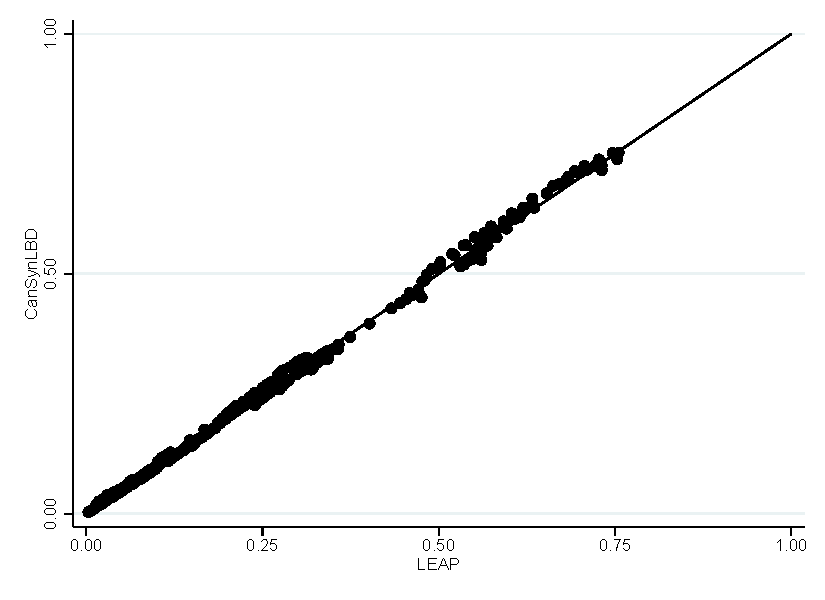
\includegraphics[height=2.8in, width=.7\linewidth]{graphs/Share_of_firms_by_NAICS_two-digit_and_year_private_bw.pdf} 
\begin{minipage}{0.85\textwidth}
{\footnotesize Note: $LEAP$ is the Longitudinal Employment Analysis Program and $CanSynLBD$ is the Canadian synthetic database based on LEAP. In this graph, we use the 2015 vintage of LEAP for the private sector and drop the last year of observation for each firm. \par}
\end{minipage}
\end{figure}


\vspace{-15.5pt}
\begin{figure} [H]
\centering
\caption{Share of firms by NAICS two-digit and year (manufacturing)} \label{FirmShareManufacturing}
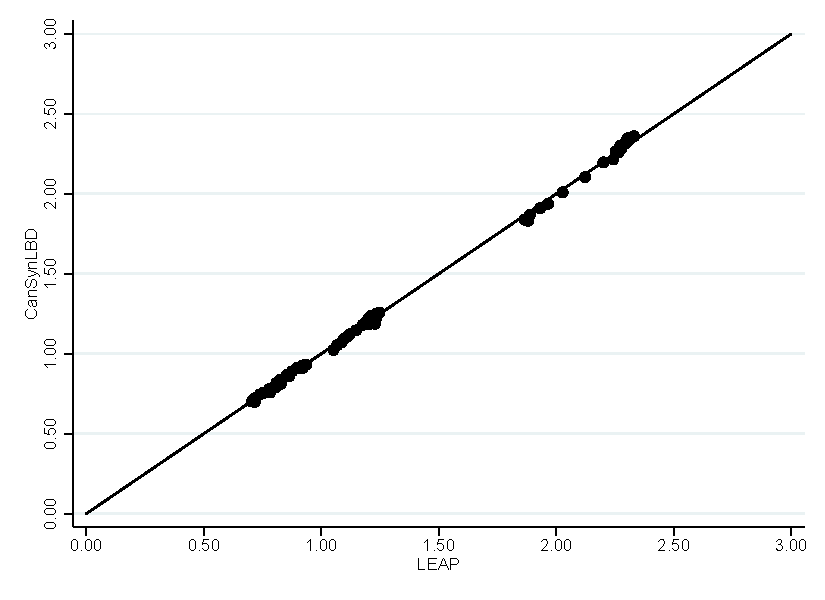
\includegraphics[height=2.8in, width=.7\linewidth]{graphs/Share_of_firms_by_NAICS_two-digit_and_year_Manufacturing_bw.pdf} 
\begin{minipage}{0.85\textwidth}
{\footnotesize Note: $LEAP$ is the Longitudinal Employment Analysis Program and $CanSynLBD$ is the Canadian synthetic database based on LEAP. In this graph, we use the 2015 vintage of LEAP for the private sector and drop the last year of observation for each firm. \par}
\end{minipage}
\end{figure}

Figures \ref{EmploymentSharePrivate} and \ref{EmploymentShareManufacturing} plot the share of employment by two-digit industry and year for both the CanSynLBD and the LEAP database
\footnote{$x_{its} = X_{its}/\sum_{i} \sum_{t} X_{its}$,\todo{BD: Define $x$ and $X$} where $i$ are two-digit NAICS industries, $t$ are the years in-sample, and $s$ indicates whether it is in the synthetic or confidential data. } and show that those shares do not cluster along the 45-degree line. However, this hides significant differences between sectors as, for the share of employment for the manufacturing sector, we do observe clustering along the 45-degrees.\todo{BD: This is not easily apparent from the graph}
\begin{figure} [H]
\centering
\caption{Share of employment by NAICS two-digit and year (private)} \label{EmploymentSharePrivate}
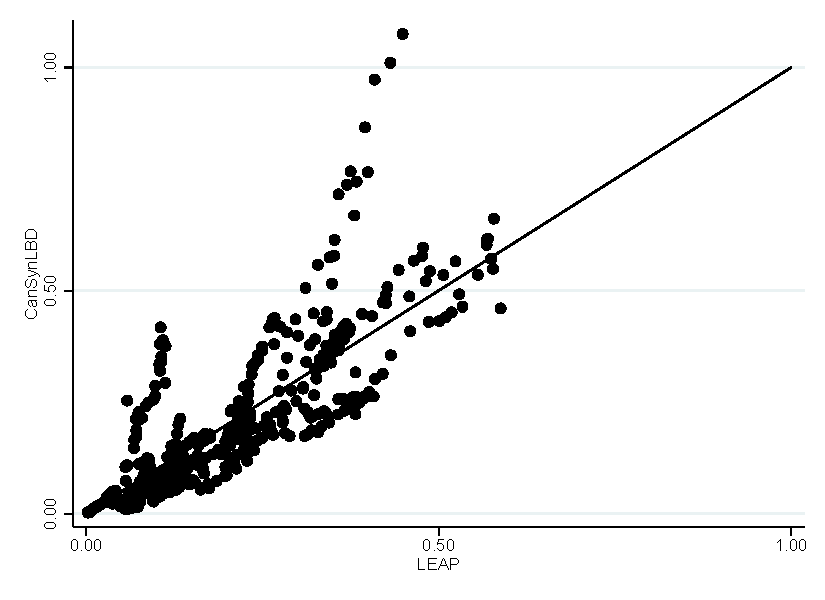
\includegraphics[height=2.8in, width=.7\linewidth]{graphs/Share_of_employment_by_NAICS_two-digit_and_year_private_bw.pdf} 
\begin{minipage}{0.85\textwidth}
{\footnotesize Note: $LEAP$ is the Longitudinal Employment Analysis Program and $CanSynLBD$ is the Canadian synthetic database based on LEAP. In this graph, we use the 2015 vintage of LEAP for the private sector and drop the last year of observation for each firm. \par}
\end{minipage}
\end{figure}
\vspace{-15.5pt}
\begin{figure} [H]
\centering
\caption{Share of employment by NAICS two-digit and year (manufacturing)} \label{EmploymentShareManufacturing}
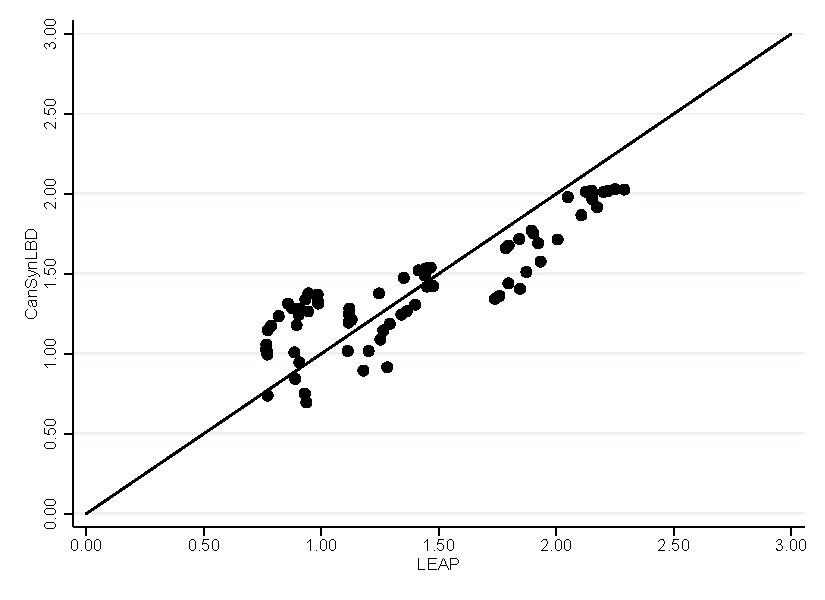
\includegraphics[height=2.8in, width=.7\linewidth]{graphs/Share_of_employment_by_NAICS_two-digit_and_year_Manufacturing_bw.pdf} 
\begin{minipage}{0.85\textwidth}
{\footnotesize Note: $LEAP$ is the Longitudinal Employment Analysis Program and $CanSynLBD$ is the Canadian synthetic database based on LEAP. In this graph, we use the 2015 vintage of LEAP for the private sector and drop the last year of observation for each firm. \par}
\end{minipage}
\end{figure}

Figures \ref{PayrollSharePrivate} and \ref{PayrollShareManufacturing} plot the share of payroll by two-digit industry and year for both CanSynLBD and LEAP database and show that those shares do not cluster along the 45-degree line. Again, we do notice that for the share of employment for the manufacturing sector, we do observe clustering along the 45-degrees.\todo{BD: This is not easily apparent from the graph}
\begin{figure} [H]
\centering
\caption{Share of payroll by NAICS two-digit and year (private)} \label{PayrollSharePrivate}
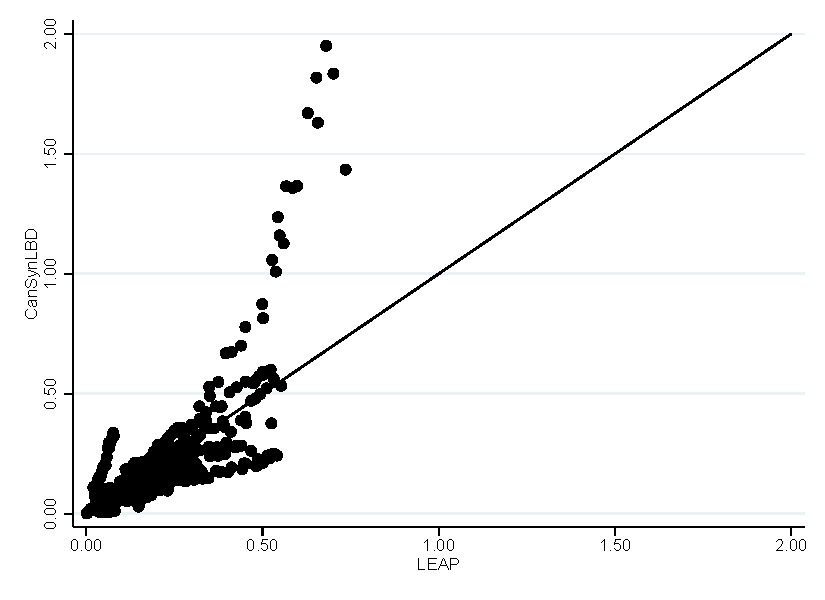
\includegraphics[height=2.8in, width=.7\linewidth]{graphs/Share_of_payroll_by_NAICS_two-digit_and_year_private_bw.pdf} 
\begin{minipage}{0.85\textwidth}
{\footnotesize Note: $LEAP$ is the Longitudinal Employment Analysis Program and $CanSynLBD$ is the Canadian synthetic database based on LEAP. In this graph, we use the 2015 vintage of LEAP for the private sector and drop the last year of observation for each firm. \par}
\end{minipage}
\end{figure}
\vspace{-15.5pt}
\begin{figure} [H]
\centering
\caption{Share of payroll by NAICS two-digit and year (manufacturing)} \label{PayrollShareManufacturing}
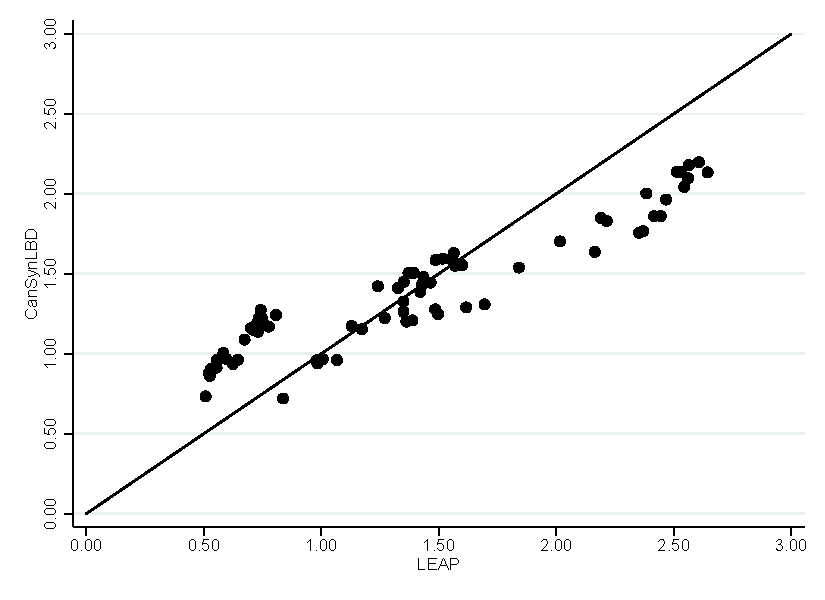
\includegraphics[height=2.8in, width=.7\linewidth]{graphs/Share_of_payroll_by_NAICS_two-digit_and_year_Manufacturing_bw.pdf} 
\begin{minipage}{0.85\textwidth}
{\footnotesize Note: $LEAP$ is the Longitudinal Employment Analysis Program and $CanSynLBD$ is the Canadian synthetic database based on LEAP. In this graph, we use the 2015 vintage of LEAP for the private sector and drop the last year of observation for each firm. \par}
\end{minipage}
\end{figure}

\subsection{Firm Dynamics}
To assess how well the CanSynLBD captures firm dynamics, we also compute entry and exit rates of the private sector by year. Table \ref{FirmDynamics} shows that those rates for CanSynLBD are similar to LEAP database. In addition, we compute the difference between the entry rate as the entry rate of CanSynLBD net the entry rate of LEAP and the divergence of exit rate as the exit rate of CanSynLBD net the exit rate of LEAP \todo{BD: I don't understand what was done here}(see Table \ref{FirmDynamics}).
\todo{LV Reformat table, compute divergence}

\begin{table}[H]
  \centering
\begin{threeparttable}
 \caption{Entry and exit rates by year} \label{FirmDynamics} \medskip
\renewcommand{\arraystretch}{1}
\begin{tabular}{l|c c| c c| c c}
\toprule
&\multicolumn{2}{c|}{\textbf{LEAP}} &  \multicolumn{2}{c|}{\textbf{CanSynLBD}}&  \multicolumn{2}{c}{\textbf{Divergence}}\\
\textbf{Year}&\textbf{Entry Rate}&\textbf{Exit Rate}&\textbf{Entry Rate}&\textbf{Exit Rate} &\textbf{Entry Rate}&\textbf{Exit Rate}\\
\midrule
1992&11.77&11.72&11.16&11.71&-0.60&-0.00\\
1993&11.81&11.61&10.84&12.18&-0.97&0.57\\
1994&12.04&11.79&11.57&12.01&-0.47&0.22\\
1995&11.94&12.09&11.69&12.26&-0.25&0.17\\
1996&12.91&10.31&12.62&10.64&-0.29&0.32\\
1997&13.18&9.75&13.03&10.21&-0.15&0.47\\
1998&12.48&10.89&12.97&10.13&0.50&-0.75\\
1999&12.00&10.66&12.16&9.97&0.16&-0.69\\
2000&11.80&10.51&11.59&9.70&-0.20&-0.82\\
2001&11.44&10.20&11.33&9.52&-0.12&-0.68\\
2002&11.39&9.91&11.10&9.03&-0.29&-0.89\\
2003&11.17&10.21&10.52&9.37&-0.65&-0.84\\
2004&12.13&9.76&10.94&9.57&-1.20&-0.20\\
2005&11.92&10.07&11.07&9.86&-0.84&-0.21\\
2006&11.81&9.96&11.15&9.34&-0.66&-0.62\\
2007&12.28&9.80&10.99&9.31&-1.29&-0.49\\
2008&11.60&10.14&10.78&9.75&-0.82&-0.40\\
2009&10.77&9.93&9.99&9.81&-0.78&-0.12\\
2010&10.80&9.75&9.91&9.65&-0.89&-0.10\\
2011&10.62&9.79&9.73&10.00&-0.89&0.21\\
2012&10.60&9.76&10.02&10.20&-0.58&0.44\\
2013&10.16&9.71&9.95&10.32&-0.21&0.62\\
2014&9.93&10.11&9.26&10.70&-0.67&0.59\\

   \bottomrule
  \end{tabular} 
\begin{tablenotes}
\small
\item Note: $LEAP$ is the Longitudinal Employment Analysis Program and $CanSynLBD$ is the Canadian synthetic database based on LEAP. In this graph, we use 2015 vintage of LEAP for the manufacturing sector and drop last year observation of each firm. We calculate the divergence of entry rate as the entry rate of CanSynLBD net the entry rate of LEAP and the divergence of exit rate as the exit rate of CanSynLBD net the exit rate of LEAP.
 \end{tablenotes}
 \end{threeparttable}
\end{table}

\begin{figure} [H]
\centering
\caption{Divergence of exit and entry rate between LEAP and CanSynLBD} \label{Divergence}
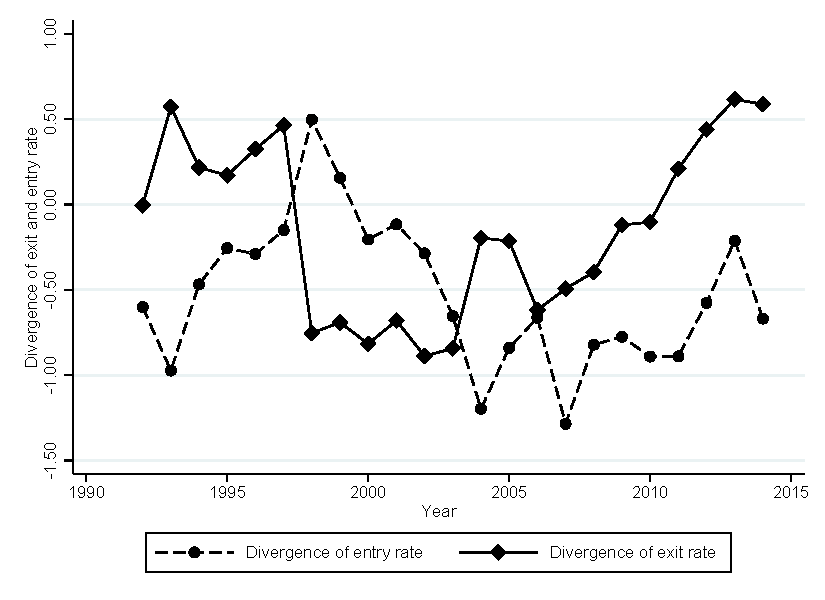
\includegraphics[height=2.8in, width=.7\linewidth]{graphs/Divergence_of_exit_and_entry_rate_between_LEAP_and_CanSynLBD_bw.pdf} 
\begin{minipage}{0.85\textwidth}
{\footnotesize Note: $LEAP$ is the Longitudinal Employment Analysis Program and $CanSynLBD$ is the Canadian synthetic database based on LEAP. In this graph, we use 2015 vintage of LEAP for private sector and drop last year observation of each firm. We calculate the divergence of entry rate as the entry rate of CanSynLBD net the entry rate of LEAP and the divergence of exit rate as the exit rate of CanSynLBD net the exit rate of LEAP. \par}
\end{minipage}
\end{figure}

\subsection{Dynamics of Job Flows}

One of the most important applications of LEAP is to generate statistics that describe job flows. Following \cite{DavisHaltiwangerSchuh}, the job creation is defined as the sum of all employment gains from expanding firms from year $t-1$ to year $t$ including entry firms. The job destruction rate is defined as the sum of all employment losses from contracted \todo{BD: Contracted?}firms from year $t-1$ to year $t$ including exiting firms. Net job creation is the job creation rate minus the job destruction rate. Figures \ref{JobCreationPrivate} and \ref{JobCreationManufacturing} show the job creation rates from the CanSynLBD compared againg those of the LEAP. These figures show that the manufacturing sector has closer pattern than the private sector. We find a similar patterns for net job creation rates (Figures \ref{NetJobCreationPrivate} and  \ref{NetJobCreationManufacturing}).

\begin{figure} [H]
\centering
\caption{Job creation rate by year (private)} \label{JobCreationPrivate}
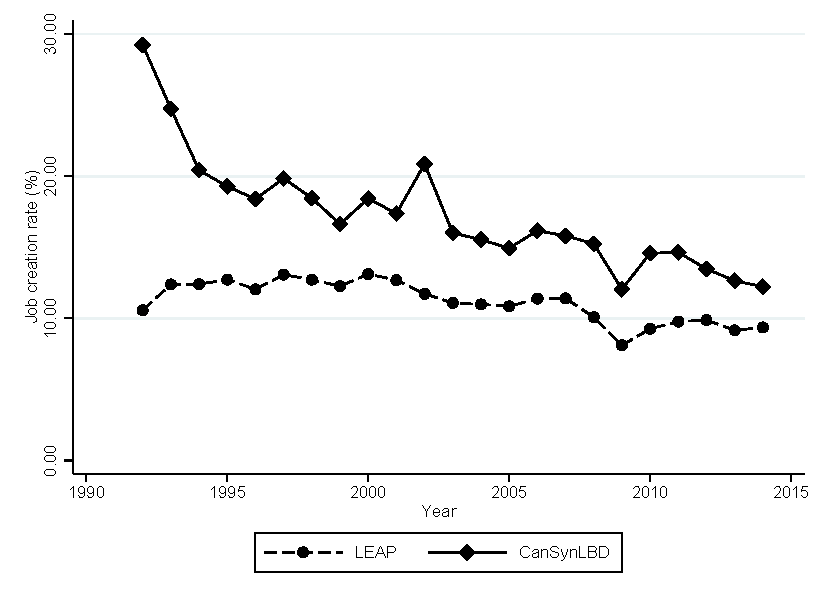
\includegraphics[height=2.8in, width=.7\linewidth]{graphs/Job_creation_rate_by_year_private_bw.pdf} 
\begin{minipage}{0.85\textwidth}
{\footnotesize Note: $LEAP$ is the Longitudinal Employment Analysis Program and $CanSynLBD$ is the Canadian synthetic database based on LEAP. In this graph, we use 2015 vintage of LEAP for the private sector and drop last year observation of each firm. \todo{BD: Make sure we use the same table footnote when appropriate; this should be \LateX coded.}\par}
\end{minipage}
\end{figure}
\begin{figure} [H]
\centering
\caption{Job creation rate  by year (manufacturing)} \label{JobCreationManufacturing}
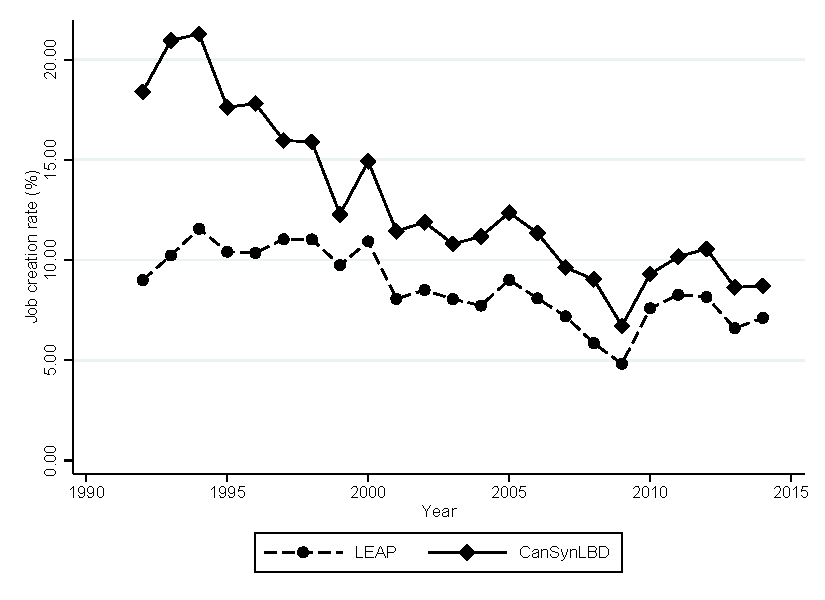
\includegraphics[height=2.8in, width=.7\linewidth]{graphs/Job_creation_rate_by_year_Manufacturing_bw.pdf} 
\begin{minipage}{0.85\textwidth}
{\footnotesize Note: $LEAP$ is the Longitudinal Employment Analysis Program and $CanSynLBD$ is the Canadian synthetic database based on LEAP. In this graph, we use 2015 vintage of LEAP for the manufacturing sector and drop last year observation of each firm. \par}
\end{minipage}
\end{figure}

\todo{LV regraph, dropping last year (net job creation not defined)}
\begin{figure} [H]
\centering
\caption{Net job creation rate by year (private)} \label{NetJobCreationPrivate}
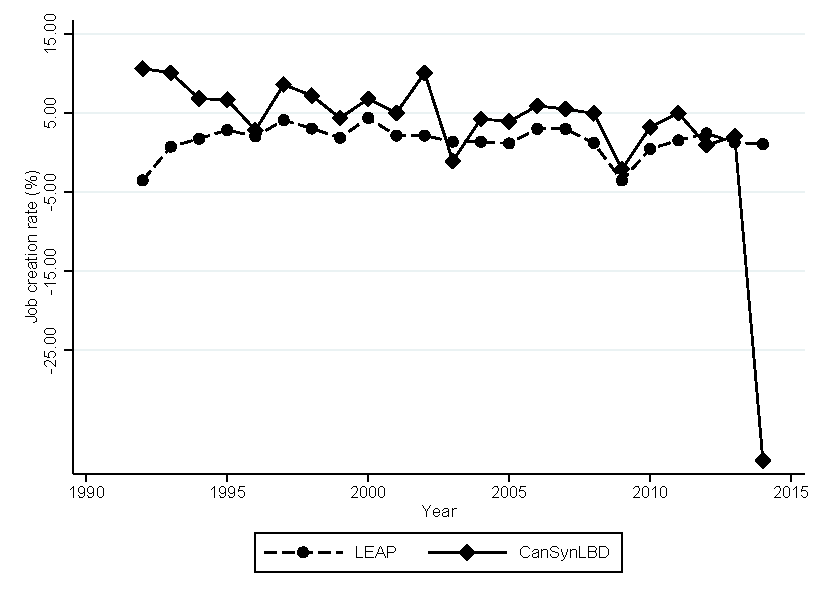
\includegraphics[height=2.8in, width=.7\linewidth]{graphs/Net_job_creation_rate_by_year_private_bw.pdf} 
\begin{minipage}{0.85\textwidth}
{\footnotesize Note: $LEAP$ is the Longitudinal Employment Analysis Program and $CanSynLBD$ is the Canadian synthetic database based on LEAP. In this graph, we use 2015 vintage of LEAP for the private sector and drop last year observation of each firm. \par}
\end{minipage}
\end{figure}
\begin{figure} [H]
\centering
\caption{Net job creation rate  by year (manufacturing)} \label{NetJobCreationManufacturing}
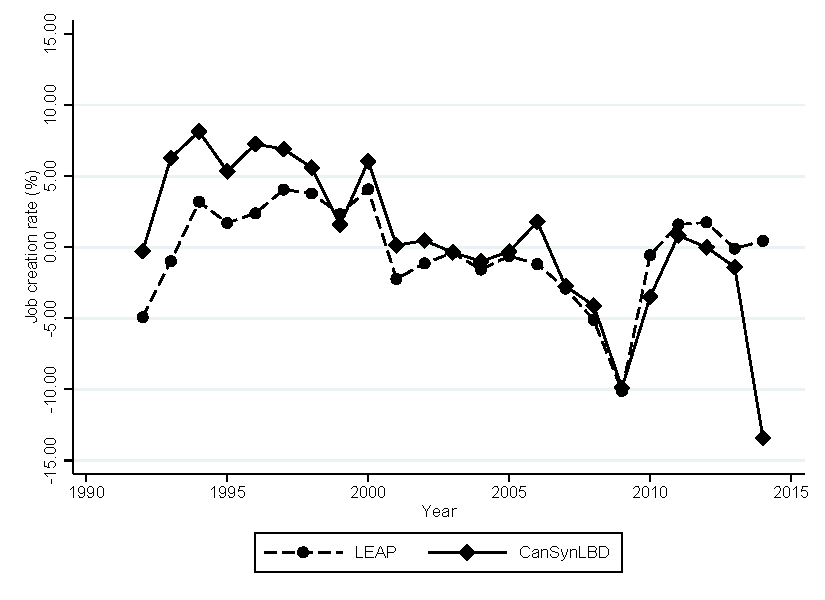
\includegraphics[height=2.8in, width=.7\linewidth]{graphs/Net_job_creation_rate_by_year_Manufacturing_bw.pdf} 
\begin{minipage}{0.85\textwidth}
{\footnotesize Note: $LEAP$ is the Longitudinal Employment Analysis Program and $CanSynLBD$ is the Canadian synthetic database based on LEAP. In this graph, we use 2015 vintage of LEAP for the manufacturing sector and drop last year observation of each firm. \par}
\end{minipage}
\end{figure}

\subsection{pMSE}

To compare the quality of the synthetic data relative to the confidential data, we compute $pMSE$, which is the mean-squared error of the predicted probabilities (i.e., propensity scores) for those two databases. Specifically, $pMSE$ is a metric to assess how well we are able to discern between synthetic data and confidential data. %This means that these two databases have high distributional similar if we are unable to discern.

We follow the method by \textcite{SnokeSlavkovic2018} to calculate the $pMSE$. This method involved the following steps: 
\begin{enumerate}
    \item Append the $n_1$ rows of the confidential database $X$ to the $n_2$ rows of the synthetic database $X^s$ to create $X^{comb}$ with $N=n_1 + n_2$ rows.
    \item Create an indicator variable, $I$, to $X^{comb}$ subject to $I=\{1: X^{comb} \in X^s\}$. This means that we create an indicator variable of $1$ for the synthetic database and $0$ for the confidential database. 
    \item Fit the following model to predict $I$
    \begin{eqnarray}	
        I & = &\alpha + ALU_{it} + \lambda Pay_{it} + Age_{it}^{T}\beta + \lambda_t + \alpha_s + \epsilon_{it} \label{pMSE}\todo{BD: I don't understand why the dependant variable has no indices?}
     \end{eqnarray}
    where $ALU_{it}$ is the logarithm of average labour unit (ALU) of firm $i$ in year $t$, $Pay_{it}$ is the logarithm of payroll of firm $i$ in year $t$, $Age_{it}$ is a vector of dummy variables for age of firm $i$ in year $t$, $\lambda_t$ is the year fixed effect, $\alpha_s$ is an unobserved time-invariant industry-specific effect, and $\epsilon_{it}$ is the disturbance term of firm $i$ in year $t$. 
    \item calculate the predicted probabilities, $\hat{p}_i$ for each row of $X^{comb}$
    \item Compute the $pMSE=\frac{1}{N}\sum_{i=1}^N(\hat{p}_i - 0.5)^2$
\end{enumerate}
A $pMSE$ = 0 means every $\hat{p}_i = 0.5$. %This implies the highest utility. 

To compute the $pMSE$, we estimate equation \ref{pMSE} using both the logit and probit models. Table \ref{pMSE_regression} \todo{BD: Are those coefficients or marginal effects? Does it make sense to show coefficients? Or are we interested only in the last row? If we are interested in the coefficient, why is there no discussion of those?} shows the calculated value of $pMSE$, which is lower for the manufacturing sector than the public sector in both regressions. This is because, as we explained before, the synthetic data mirrors the original data more closely in the case of the manufacturing sector.

\begin{table}[H]
  \centering
\begin{threeparttable}
 \caption{pMSE estimates} \label{pMSE_regression} \medskip
\renewcommand{\arraystretch}{1}
\begin{tabular}{l|c c| c c}
\toprule
\textbf{Independent Variables}&\multicolumn{2}{c|}{\textbf{Logistic Regression}} &  \multicolumn{2}{c}{\textbf{Probit Regression}}\\
\midrule
          &\multicolumn{1}{c}{Manufacturing}&\multicolumn{1}{c}{Private}&\multicolumn{1}{c}{Manufacturing}&\multicolumn{1}{c}{Private}\\
\hline
Ln ALU    &   0.1580\sym{***}&   0.7138\sym{***}&   0.1003\sym{***}&   0.4390\sym{***}\\
          & (0.0039)         & (0.0010)         & (0.0024)         & (0.0006)         \\
[1em]
Ln Pay    &   0.0039         &  -0.4426\sym{***}&   0.0012         &  -0.2691\sym{***}\\
          & (0.0037)         & (0.0010)         & (0.0023)         & (0.0006)         \\
[1em]
Age 3-4   &   0.0392\sym{***}&   0.0972\sym{***}&   0.0252\sym{***}&   0.0618\sym{***}\\
          & (0.0078)         & (0.0017)         & (0.0049)         & (0.0010)         \\
[1em]
Age 5-7   &  -0.0382\sym{***}&   0.0477\sym{***}&  -0.0233\sym{***}&   0.0309\sym{***}\\
          & (0.0073)         & (0.0016)         & (0.0045)         & (0.0010)         \\
[1em]
Age 8-12  &  -0.1258\sym{***}&  -0.0263\sym{***}&  -0.0781\sym{***}&  -0.0152\sym{***}\\
          & (0.0071)         & (0.0015)         & (0.0044)         & (0.0009)         \\
[1em]
Age 13 or more&  -0.2190\sym{***}&  -0.1024\sym{***}&  -0.1365\sym{***}&  -0.0627\sym{***}\\
          & (0.0074)         & (0.0016)         & (0.0046)         & (0.0010)         \\
\hline
\(N\)     &  2243011         & 34638723         &  2243011         & 34638723         \\
pseudo \(R^{2}\)&   0.0112         &   0.0318         &   0.0112         &   0.0320         \\
pMSE      &   0.0041         &   0.0121         &   0.0041         &   0.0124         \\

   \bottomrule
  \end{tabular} 
\begin{tablenotes}
\small
\item Note: An observation is a firm and a year of both synthetic and original databases. In all specifications, we include both time and industry fixed effects. Standard errors are in parentheses. In this table, we use 2015 vintage of LEAP to create the synthetic database and drop last year observation of each firm. ***, **, and * indicate statistically significant coefficients at 1\%, 5\%, and 10\% percent levels, respectively.
 \end{tablenotes}
 \end{threeparttable}
\end{table}

\subsection{Regression Analysis}

To assess how well the CanSynLBD captures variability in economic growth due to industry and firm age, we estimate the following dynamic panel data model:
\begin{eqnarray}	
ALU_{it} & = & \alpha + \theta ALU_{i,t-1} + \lambda Pay_{it} + Age_{it}^{T}\beta + \lambda_t + \alpha_s + \epsilon_{it}
\end{eqnarray}
where $ALU_{it}$ is the logarithm of average labour unit (ALU) of firm $i$ in year $t$, $ALU_{i,t-1}$ is the logarithm of last year's average labour unit (ALU) of firm $i$, $Pay_{it}$ is the logarithm of payroll of firm $i$ in year $t$, $Age_{it}$ is a vector of dummy variables for age of firm $i$ in year $t$, $\lambda_t$ is the year fixed effect, $\alpha_s$ is an unobserved time-invariant industry-specific effect, and $\epsilon_{it}$ is the disturbance term of firm $i$ in year $t$. 

\begin{table}[H]
  \centering
\begin{threeparttable}
 \caption{Regression coefficients (OLS)} \label{OLS} \medskip
\renewcommand{\arraystretch}{1}
\begin{tabular}{l|c c| c c}
\toprule
\textbf{Independent Variables}&\multicolumn{2}{c|}{\textbf{LEAP}} &  \multicolumn{2}{c}{\textbf{CanSynLBD}}\\
\midrule
&\multicolumn{1}{c}{Private}&\multicolumn{1}{c}{Manufacturing}&\multicolumn{1}{c}{Private}&\multicolumn{1}{c}{Manufacturing}\\
\hline
AR(1) Coefficient&   0.2031\sym{***}&   0.2481\sym{***}&   0.3970\sym{***}&   0.4405\sym{***}\\
          & (0.0001)         & (0.0005)         & (0.0002)         & (0.0007)         \\
[1em]
Ln Pay    &   0.7847\sym{***}&   0.7300\sym{***}&   0.5481\sym{***}&   0.5228\sym{***}\\
          & (0.0001)         & (0.0005)         & (0.0002)         & (0.0006)         \\
[1em]
Age 3-4   &  -0.1202\sym{***}&  -0.1717\sym{***}&  -0.1223\sym{***}&  -0.2340\sym{***}\\
          & (0.0003)         & (0.0014)         & (0.0004)         & (0.0016)         \\
[1em]
Age 5-7   &  -0.1260\sym{***}&  -0.1891\sym{***}&  -0.1235\sym{***}&  -0.2507\sym{***}\\
          & (0.0003)         & (0.0014)         & (0.0004)         & (0.0016)         \\
[1em]
Age 8-12  &  -0.1268\sym{***}&  -0.1973\sym{***}&  -0.1169\sym{***}&  -0.2551\sym{***}\\
          & (0.0003)         & (0.0013)         & (0.0004)         & (0.0016)         \\
[1em]
Age 13 or more&  -0.1246\sym{***}&  -0.1992\sym{***}&  -0.1101\sym{***}&  -0.2577\sym{***}\\
          & (0.0003)         & (0.0014)         & (0.0004)         & (0.0017)         \\
\hline
\(N\)     & 15708195         &  1015293         & 13573225         &   959764         \\
\(R^{2}\) &   0.9696         &   0.9743         &   0.9444         &   0.9523         \\

   \bottomrule
  \end{tabular} 
\begin{tablenotes}
\small
\item Note: In all specifications, we include both year and industry fixed effects. Standard errors are in parentheses. $LEAP$ is the Longitudinal Employment Analysis Program and $CanSynLBD$ is the Canadian synthetic database based on LEAP. In this table, we use the 2015 vintage of LEAP and drop last year observation of each firm. ***, **, and * indicate statistically significant coefficients at 1\%, 5\%, and 10\% percent levels, respectively.
 \end{tablenotes}
 \end{threeparttable}
\end{table}

We estimate the model separately on LEAP and CanSynLBD data for the private and manufacturing sectors and find that the CansynLBD data provides similar predictions to LEAP data (Tables  \ref{OLS}).\todo{compute overlap interval}

\begin{table}[H]
  \centering
\begin{threeparttable}
 \caption{Regression coefficients (Dynamic)} \label{Dynamic - GMM} \medskip
\renewcommand{\arraystretch}{1}
\begin{tabular}{l|c c| c c}
\toprule
\textbf{Independent Variables}&\multicolumn{2}{c|}{\textbf{LEAP}} &  \multicolumn{2}{c}{\textbf{CanSynLBD}}\\
\midrule
&\multicolumn{1}{c}{Private}&\multicolumn{1}{c}{Manufacturing}&\multicolumn{1}{c}{Private}&\multicolumn{1}{c}{Manufacturing}\\
\hline
AR(1) Coefficient&   0.0805\sym{***}&   0.1189\sym{***}&   0.5722\sym{***}&   0.5425\sym{***}\\
          & (0.0003)         & (0.0018)         & (0.0024)         & (0.0084)         \\
[1em]
Ln Pay    &   0.8991\sym{***}&   0.8523\sym{***}&   0.4101\sym{***}&   0.4302\sym{***}\\
          & (0.0002)         & (0.0015)         & (0.0018)         & (0.0067)         \\
[1em]
Age 3-4   &  -0.0450\sym{***}&  -0.0797\sym{***}&  -0.2075\sym{***}&  -0.2972\sym{***}\\
          & (0.0002)         & (0.0014)         & (0.0010)         & (0.0051)         \\
[1em]
Age 5-7   &  -0.0438\sym{***}&  -0.0860\sym{***}&  -0.2129\sym{***}&  -0.3162\sym{***}\\
          & (0.0002)         & (0.0015)         & (0.0011)         & (0.0059)         \\
[1em]
Age 8-12  &  -0.0418\sym{***}&  -0.0923\sym{***}&  -0.2187\sym{***}&  -0.3294\sym{***}\\
          & (0.0003)         & (0.0017)         & (0.0013)         & (0.0070)         \\
[1em]
Age 13 or more&  -0.0379\sym{***}&  -0.0898\sym{***}&  -0.2318\sym{***}&  -0.3414\sym{***}\\
          & (0.0003)         & (0.0019)         & (0.0015)         & (0.0080)         \\
\hline
\(N\)     & 15708195         &  1015293         & 13573225         &   959764         \\
m2        & -14.5000         &  -2.2200         & -27.5400         &  -9.4400         \\
Sargan test&  6.9e+04         &  4.6e+03         &  1.5e+04         &  1.5e+03         \\
df of Sargan Test& 252.0000         & 252.0000         & 252.0000         & 252.0000         \\
P value of Sargan test&   0.0000         &   0.0000         &   0.0000         &   0.0000         \\

   \bottomrule
  \end{tabular} 
\begin{tablenotes}
\small
\item Note: In this table, $m2$ is the Arellano-Bond test for zero autocorrelation in first-differenced errors for order two. $LEAP$ is the Longitudinal Employment Analysis Program and $CanSynLBD$ is the Canadian synthetic database based on LEAP. In this graph, we use the 2015 vintage of LEAP and drop last year observation of each firm. Standard errors are in parentheses. ***, **, and * indicate statistically significant coefficients at 1\%, 5\%, and 10\% percent levels, respectively.
 \end{tablenotes}
 \end{threeparttable}
\end{table}

As $ALU_{st-1}$ is correlated with $\alpha_{s}$ because $ALU_{st-1}$ is a function of $\alpha_{s}$, OLS estimators are biased and inconsistent. 
To take this endogeneity bias into account, we use the estimation method from \textcite{RePEc:oup:restud:v:58:y:1991:i:2:p:277-297.} and find similar predictions (Table \ref{Dynamic - GMM}). To check the validity of the model, we use two tests. First, to test for autocorrelation, we use the test $m2$ by \textcite{RePEc:oup:restud:v:58:y:1991:i:2:p:277-297.}. In the table, we report the $z$ test statistic for $m2$ test for zero autocorrelation in the  first-differenced errors of order two. Second, we use the Sargan test to verify the validity of instrument subsets (showned in the last three rows in the table).

We furthermore estimate the model using the system GMM  method proposed by \textcite{RePEc:eee:econom:v:68:y:1995:i:1:p:29-51} and \textcite{RePEc:eee:econom:v:87:y:1998:i:1:p:115-143} and find similar predictions as before (Table \ref{Dynamic - system GMM}). 

\begin{table}[H]
  \centering
\begin{threeparttable}
 \caption{Regression coefficients (Dynamic - system GMM)} \label{Dynamic - system GMM} \medskip
\renewcommand{\arraystretch}{1}
\begin{tabular}{l|c c| c c}
\toprule
\textbf{Independent Variables}&\multicolumn{2}{c|}{\textbf{LEAP}} &  \multicolumn{2}{c}{\textbf{CanSynLBD}}\\
\midrule
&\multicolumn{1}{c}{Private}&\multicolumn{1}{c}{Manufacturing}&\multicolumn{1}{c}{Private}&\multicolumn{1}{c}{Manufacturing}\\
\hline
AR(1) Coefficient&   0.0978\sym{***}&   0.1614\sym{***}&   0.5111\sym{***}&   0.5780\sym{***}\\
          & (0.0002)         & (0.0014)         & (0.0008)         & (0.0041)         \\
[1em]
Ln Pay    &   0.8854\sym{***}&   0.8161\sym{***}&   0.4562\sym{***}&   0.4022\sym{***}\\
          & (0.0002)         & (0.0012)         & (0.0006)         & (0.0033)         \\
[1em]
Age 3-4   &  -0.0555\sym{***}&  -0.1097\sym{***}&  -0.1828\sym{***}&  -0.3177\sym{***}\\
          & (0.0002)         & (0.0012)         & (0.0004)         & (0.0028)         \\
[1em]
Age 5-7   &  -0.0558\sym{***}&  -0.1201\sym{***}&  -0.1860\sym{***}&  -0.3408\sym{***}\\
          & (0.0002)         & (0.0013)         & (0.0005)         & (0.0031)         \\
[1em]
Age 8-12  &  -0.0548\sym{***}&  -0.1298\sym{***}&  -0.1875\sym{***}&  -0.3583\sym{***}\\
          & (0.0002)         & (0.0014)         & (0.0005)         & (0.0036)         \\
[1em]
Age 13 or more&  -0.0524\sym{***}&  -0.1317\sym{***}&  -0.1943\sym{***}&  -0.3747\sym{***}\\
          & (0.0002)         & (0.0016)         & (0.0006)         & (0.0041)         \\
\hline
\(N\)     & 15708195         &  1015293         & 13573225         &   959764         \\
m2        & -11.4300         &   1.3900         & -41.6000         &  -7.6700         \\
Sargan test&  7.7e+04         &  6.3e+03         &  1.8e+04         &  1.7e+03         \\
df of Sargan Test& 274.0000         & 274.0000         & 274.0000         & 274.0000         \\
P value of Sargan test&   0.0000         &   0.0000         &   0.0000         &   0.0000         \\

   \bottomrule
  \end{tabular} 
\begin{tablenotes}
\small
\item Note: An observation is a firm and a year. In this table, $m2$ is the Arellano-Bond test for zero autocorrelation in first-differenced errors for order two. $LEAP$ is the Longitudinal Employment Analysis Program and $CanSynLBD$ is the Canadian synthetic database based on LEAP. In this table, we use 2015 vintage of LEAP and drop last year observation of each firm. Standard errors are in parentheses. ***, **, and * indicate statistically significant coefficients at 1\%, 5\%, and 10\% percent levels, respectively.
 \end{tablenotes}
 \end{threeparttable}
\end{table}

We also estimate above dynamic panel data model with a first-order moving average using appropriate instruments for both level and difference equation as proposed by \textcite{RePEc:eee:econom:v:68:y:1995:i:1:p:29-51} and \textcite{RePEc:eee:econom:v:87:y:1998:i:1:p:115-143}:
\begin{eqnarray}	
ALU_{it}&=&\alpha +\theta ALU_{i,t-1}+\lambda Pay_{it}+Age_{it}^{T}\beta+\lambda_t+\alpha_s+\epsilon_{it}+\gamma\epsilon_{it-1}
\end{eqnarray}

Table \ref{Dynamic - system GMM with MA(1)} shows that the CansynLBD provides similar predictions to the LEAP.

\begin{table}[H]
  \centering
\begin{threeparttable}
 \caption{Regression coefficients (Dynamic - system GMM with MA(1))} \label{Dynamic - system GMM with MA(1)} \medskip
\renewcommand{\arraystretch}{1}
\begin{tabular}{l|c c| c c}
\toprule
\textbf{Independent Variables}&\multicolumn{2}{c|}{\textbf{LEAP}} &  \multicolumn{2}{c}{\textbf{CanSynLBD}}\\
\midrule
&\multicolumn{1}{c}{Private}&\multicolumn{1}{c}{Manufacturing}&\multicolumn{1}{c}{Private}&\multicolumn{1}{c}{Manufacturing}\\
\hline
AR(1) Coefficient&   0.2005\sym{***}&   0.2821\sym{***}&   0.4850\sym{***}&   0.5737\sym{***}\\
          & (0.0007)         & (0.0040)         & (0.0012)         & (0.0059)         \\
[1em]
Ln Pay    &   0.8044\sym{***}&   0.7135\sym{***}&   0.4760\sym{***}&   0.4056\sym{***}\\
          & (0.0005)         & (0.0034)         & (0.0009)         & (0.0046)         \\
[1em]
Age 3-4   &  -0.1245\sym{***}&  -0.2033\sym{***}&  -0.1716\sym{***}&  -0.3158\sym{***}\\
          & (0.0005)         & (0.0032)         & (0.0006)         & (0.0037)         \\
[1em]
Age 5-7   &  -0.1328\sym{***}&  -0.2264\sym{***}&  -0.1733\sym{***}&  -0.3389\sym{***}\\
          & (0.0005)         & (0.0035)         & (0.0006)         & (0.0043)         \\
[1em]
Age 8-12  &  -0.1383\sym{***}&  -0.2454\sym{***}&  -0.1731\sym{***}&  -0.3560\sym{***}\\
          & (0.0006)         & (0.0039)         & (0.0007)         & (0.0051)         \\
[1em]
Age 13 or more&  -0.1441\sym{***}&  -0.2586\sym{***}&  -0.1774\sym{***}&  -0.3717\sym{***}\\
          & (0.0006)         & (0.0042)         & (0.0008)         & (0.0058)         \\
\hline
\(N\)     & 15708195         &  1015293         & 13573225         &   959764         \\
m2        &   8.2000         &   7.0600         & -40.0300         &  -6.6400         \\
Sargan test&  2.8e+04         &  2.3e+03         &  1.7e+04         &  1.3e+03         \\
df of Sargan Test& 251.0000         & 251.0000         & 251.0000         & 251.0000         \\
P value of Sargan test&   0.0000         &   0.0000         &   0.0000         &   0.0000         \\

   \bottomrule
  \end{tabular} 
\begin{tablenotes}
\small
\item Note: An observation is a firm and a year. In this table, $m2$ is the Arellano-Bond test for zero autocorrelation in first-differenced errors for order two. $LEAP$ is the Longitudinal Employment Analysis Program and $CanSynLBD$ is the Canadian synthetic database based on LEAP. In this table, we use 2015 vintage of LEAP and drop last year observation of each firm. Standard errors are in parentheses. ***, **, and * indicate statistically significant coefficients at 1\%, 5\%, and 10\% percent levels, respectively.
 \end{tablenotes}
 \end{threeparttable}
\end{table}

\subsection{Confidentiality protection}

In this section, we estimate the probability that the synthetic first year equals the true first year, given the synthetic first year.\todo{BD: That is some strange wording} Tables \ref{ProbabilityPrivate} and \ref{ProbabilityManufacturing} show that these probabilities are quite low except for the first year.\todo{BD: Are we worried about this?} This is because of censoring and lack of previous information.

\begin{table}[H]
\centering\footnotesize
\caption{Observed firm births given synthetic births (private)} \label{ProbabilityPrivate} \medskip
\renewcommand{\arraystretch}{1}
\begin{tabular}{c c| c c c}
\toprule
\multicolumn{2}{c|}{\textbf{First (Birth) Year}} &  \multicolumn{3}{c}{\textbf{\% of Births over NAICS}}\\
\textbf{Synthetic}&\textbf{Actual}&\textbf{Minimum}&\textbf{Mean}&\textbf{Maximum}\\
\midrule
1991&1991&0.00&27.69&83.02\\
1992&1992&0.00&3.37&11.11\\
1993&1993&0.00&3.79&33.33\\
1994&1994&0.00&3.73&33.33\\
1995&1995&0.00&3.86&20.00\\
1996&1996&0.00&4.25&33.33\\
1997&1997&0.00&4.10&16.94\\
1998&1998&0.00&4.41&25.00\\
1999&1999&0.00&4.23&33.33\\
2000&2000&0.00&3.41&25.00\\
2001&2001&0.00&2.73&22.22\\
2002&2002&0.00&2.65&25.00\\
2003&2003&0.00&2.22&10.00\\
2004&2004&0.00&2.60&17.86\\
2005&2005&0.00&2.71&20.00\\
2006&2006&0.00&2.83&50.00\\
2007&2007&0.00&2.90&33.33\\
2008&2008&0.00&2.38&20.00\\
2009&2009&0.00&2.47&50.00\\
2010&2010&0.00&2.12&33.33\\
2011&2011&0.00&2.65&50.00\\
2012&2012&0.00&2.41&20.00\\
2013&2013&0.00&2.48&25.00\\
2014&2014&0.00&2.23&20.00\\
2015&2015&0.00&2.15&33.33\\

\bottomrule
\end{tabular} 
\\
\justify
%Note:
\end{table}

\begin{table}[H]
\centering\footnotesize
\caption{Observed firm births given synthetic births (manufacturing)} \label{ProbabilityManufacturing} \medskip
\renewcommand{\arraystretch}{1}
\begin{tabular}{c c| c c c}
\toprule
\multicolumn{2}{c|}{\textbf{First (Birth) Year}} &  \multicolumn{3}{c}{\textbf{\% of Births over NAICS}}\\
\textbf{Synthetic}&\textbf{Actual}&\textbf{Minimum}&\textbf{Mean}&\textbf{Maximum}\\
\midrule
1991&1991&4.76&31.64&52.03\\
1992&1992&0.00&3.32&10.53\\
1993&1993&0.00&3.97&33.33\\
1994&1994&0.00&4.21&33.33\\
1995&1995&0.00&4.41&20.00\\
1996&1996&0.00&5.36&33.33\\
1997&1997&0.00&4.09&16.94\\
1998&1998&0.00&5.46&25.00\\
1999&1999&0.00&5.27&33.33\\
2000&2000&0.00&3.39&25.00\\
2001&2001&0.00&2.19&10.00\\
2002&2002&0.00&2.45&25.00\\
2003&2003&0.00&1.71&10.00\\
2004&2004&0.00&2.07&17.86\\
2005&2005&0.00&1.92&16.67\\
2006&2006&0.00&2.49&50.00\\
2007&2007&0.00&1.74&14.29\\
2008&2008&0.00&1.60&20.00\\
2009&2009&0.00&1.60&20.00\\
2010&2010&0.00&1.34&33.33\\
2011&2011&0.00&2.43&50.00\\
2012&2012&0.00&1.93&20.00\\
2013&2013&0.00&1.61&20.00\\
2014&2014&0.00&1.71&14.29\\
2015&2015&0.00&1.41&14.29\\

\bottomrule
\end{tabular} 
\\
\justify
%Note:
\end{table}

\begin{figure} [H]
\centering
\caption{The difference between first and last year given synthetic first year} \label{SyntheticFirstYear}
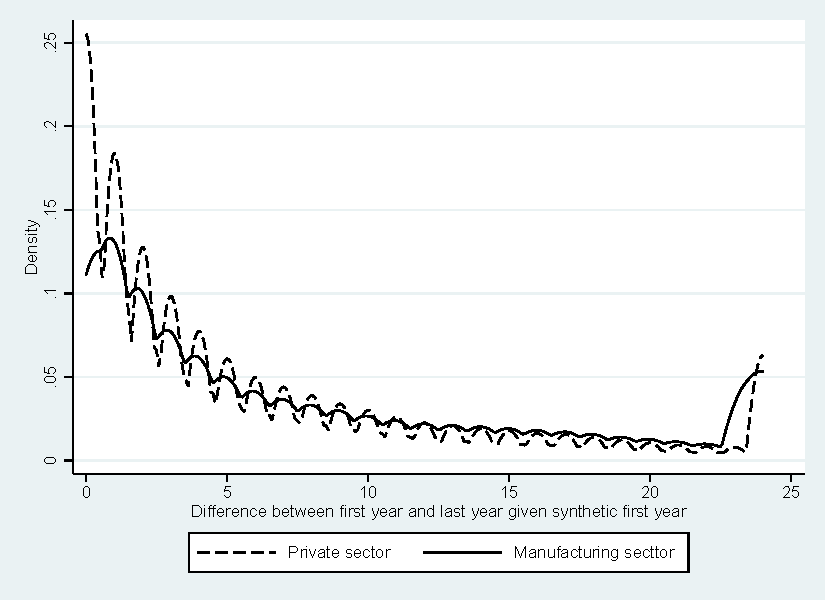
\includegraphics[height=2.8in, width=.7\linewidth]{graphs/The_difference_between_first_and_last_year_given_synthetic_first_year_bw.pdf} 
\begin{minipage}{0.85\textwidth}
%{\footnotesize Note:  \par}
\end{minipage}
\end{figure}

\section{Conclusion and Extensions}

%Statistics Canada disseminates business data in highly aggregated forms. To get access to Canadian micro business databases, 
In this paper, we adapt and implement algorithms used to create the U.S. synthetic data for LBD to create Canadian synthetic data for LEAP. We show the newly created data set is analytically valid for a wide range of statistical analyses,  as well as provide evidence on confidentiality properties.

\subsection{Addition of variables that are not analytically valid}\todo{BD: ?}

\subsection{Addition of analytically valid variables}\todo{BD: ?}

Capital stock or revenue for incorporated \todo{BD: ?}

\newpage

\appendix{Supplementary Graphs}

\section{Analytical validity}

\subsection{Confidence interval for gross employment and other measures}
We compute the standard error for gross employment as follows. We consider gross employment $E$ to be the sum of firm employments $E_j$:

\begin{equation}
E = \sum_j E_j
\end{equation}

Average firm employment $\bar{E} = \frac{E}{N_j}$ is assumed to be normally distributed, with standard deviation $\sigma_{\bar{E}}$. We compare the synthetic and the confidential data for gross employment, including error bands.

\subsection{Confidence interval overlap measures}

More generally, the question as to the statistical precision of the results obtained from the synthetic data can be assessed. For this purpose, we computed the overlap of parameter estimates  as suggested by \cite{tas2006}. We compute the \emph{interval overlap measure} $J_{k,m}$ for parameter $k$ in model $m$. Consider the overlap of confidence intervals $(L,U)$ for $\beta_{k,m}$ (estimated from the confidential data) and $(L^{*},U^{*})$ for $\beta_{k,m}^*$ (from the synthetic data). Let $L^{over} = \max (L,L^{*} )$ and $U^{over} = \min (U,U^{*})$. Then the average overlap in confidence intervals is
$$
J_{k,m}^{*} = \frac{1}{2} \left [ \frac{U^{over} - L^{over}}{U-L} + \frac{U^{over} - L^{over}}{U^*-L ^*}        \right ]
$$
We then average $J_{k,m}^{*}$ over all estimated models and parameters, by validation request. The correct counterfactual involved running these validation requests against synthetic data that does not claim analytical validity, such as synthetic data generated from uni-dimensional distributions of variables. Results are pending.\todo{BD: ?}

\subsection{Other models}

Possible papers:
\begin{itemize}
\item %\textcite{10.1257/aer.20141280} use the BDS to show the role of firm size in firm dynamics, but also had access to the Synthetic LBD.
\item \textcite{NBERc0480} use a cross-country dataset to study average post-entry behavior of young firms. 
\end{itemize}

%\bibliographystyle{apalike}
%\bibliography{paper}

\printbibliography

\end{document}